\section{非理想流动模型}


\begin{frame}
    \frametitle{非理想流动模型}

    \begin{enumerate}
        \item 离析流模型
        
        假如反应器内的流体粒子之间不存在任何形式的物质交换，那么流体粒子就像一个有边界的个体，从反应器的进口向出口运动，这样的流动叫做离析流。
        \item 多釜串联模型
        
        用N个全混釜串联来模拟一个实际的反应器。
        \item 轴向扩散模型
        
        由于分子扩散、涡流扩散以及流速分布的不均匀等原因，而使流动状况偏离理想流动时，可用轴向扩散模型来模拟，这对于管式反应器尤为合适。
    \end{enumerate}

\end{frame}


\begin{frame}
    \frametitle{离析流模型}

    \begin{minipage}{0.58\linewidth}
        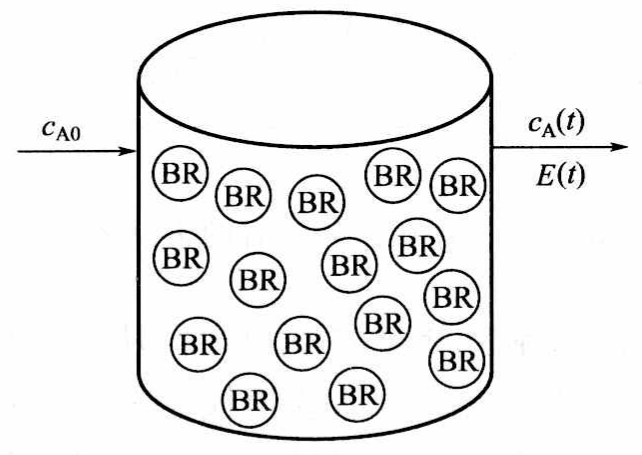
\includegraphics[width=\linewidth]{figures/fig5.16.png}
    \end{minipage}\hfill
    \begin{minipage}{0.38\linewidth}
        \begin{itemize}
            \item 假定流体粒子之间不发生微观混合
            \item BR可看作由反应物粒子群构成的间歇反应器
            \item 每个间歇反应器的反应时间取决于它们在连续流动反应器中的停留时间
        \end{itemize}
    \end{minipage}

\end{frame}


\begin{frame}
    \frametitle{离析流模型}

    根据反应器的停留时间分布知，停留时间在$t$到$t+\dif t$间的流体粒子所占的分率为$E(t)\dif t$，则这部分流体对反应器出口流体中A的浓度$\bar c_\mathrm{A}$的贡献应为$c_\mathrm{A}(t)E(t)\dif t$，将所有这些贡献相加即得反应器出口处A的平均浓度$\bar c_\mathrm{A}$，即
    \[
        \bar c_\mathrm{A} = \int_0^\infty c_\mathrm{A}(t)E(t)\dif t
    \]
    根据$c_\mathrm{A} = c_\mathrm{A0}(1 - X_\mathrm{A})$，上式可改写成
    \[
        1 - \bar X_\mathrm{A} = \int_0^\infty [1 - X_\mathrm{A}(t)]E(t)\dif t = \int_0^\infty E(t)\dif t - \int_0^\infty X_\mathrm{A}(t)E(t)\dif t
    \]
    所以
    \[
        \bar X_\mathrm{A} = \int_0^\infty X_\mathrm{A}(t)E(t)\dif t
    \]
    使用时要注意积分上限的使用（应为完全反应时间）。

\end{frame}


\begin{frame}[t]
    \frametitle{}

    \begin{example}
        等温下在反应体积为\SI{4.55}{m^3}的流动反应器中进行液相反应
        \[
            \ch{2 A -> R + P}
        \]
        该反应为二级反应，反应温度下反应速率常数$k =$\SI{2.4e-3}{m^3.mol^{-1}.min^{-1}}。进料流量为\SI{0.53}{m^3.min^{-1}}，A的浓度等于\SI{1.6}{kmol.m^{-3}}。该反应器的停留时间分布如下表所示。试计算反应器出口处A的转化率：（1）用离析流模型；（2）用活塞流模型。
        \begin{table}[]            
            \begin{tabular}{cccccccccccccc}
            \hline
            $t/\mathrm{min}$ & 0 & 2 & 4 & 6 & 8 & 10 & 12 & 14 & 16 & 18 & 20 & 22 & 24 \\ \hline
            $c /\mathrm{(g/m^3)}$ & 0 & 1 & 4 & 7 & 9 & 8 & 5 & 2 & 1.5 & 1 & 0.6 & 0.2 & 0 \\ \hline
            \end{tabular}
            \end{table}
    \end{example}

\end{frame}


\begin{frame}
    \frametitle{多釜串联模型}

    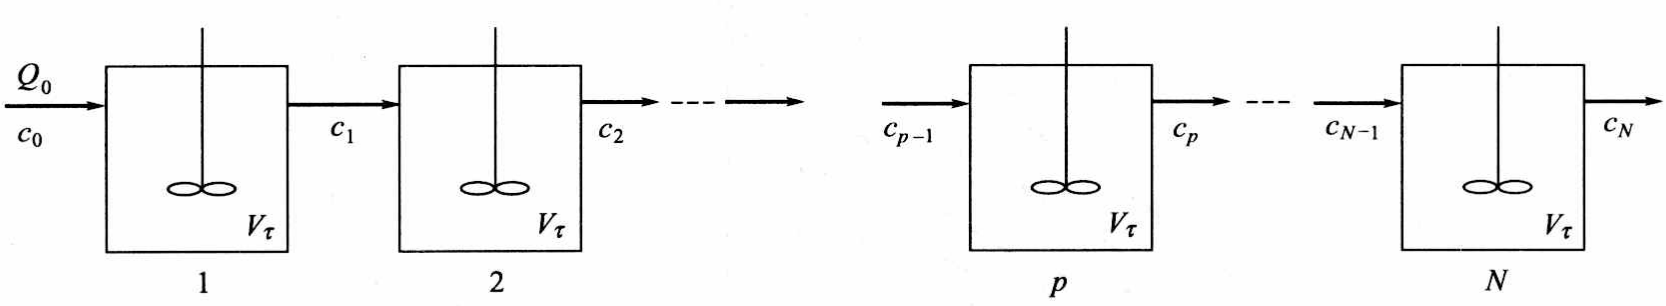
\includegraphics[width=\linewidth]{figures/fig5.17.png}

    可以用$N$个全混釜串联来模拟一个实际的反应器。$N$为模型参数。
    \begin{itemize}
        \item $N=1$时为全混流；
        \item $N=\infty$则为活塞流。
    \end{itemize}
    $N$的取值不同反映了实际反应器的不同返混程度，其具体数值由停留时间分布确定。

    为此，首先求定多釜串联时的停留时间分布。

\end{frame}


\begin{frame}
    \frametitle{多釜串联模型}

    对第$p$釜作示踪剂的物料衡算得
    \[
        Q c_{p-1}(t)-Q c_{p}(t)=V_{\mathrm{r}} \frac{\mathrm{d} c_{\mathrm{p}}(t)}{\mathrm{d} t}
    \]
    \[
        \text{或} \qquad \frac{\mathrm{d} c_{p}(t)}{\mathrm{d} t}=\frac{1}{\tau}\left[c_{p-1}(t)-c_{p}(t)\right]  \qquad
    \]
    若示踪剂呈阶跃输入，且浓度为$c_0$，则上式的初始条件为$t=0 \quad c_{p}(0)=0 \quad(p=1,2, \cdots, N)$。

    当$p=1$时，
    \[
        \frac{\mathrm{d} c_{1}(t)}{\mathrm{d} t}=\frac{1}{\tau}\left[c_{0}(t)-c_{1}(t)\right]
    \]
    此即第1釜的物料衡算式，其解为
    \[
        c_{1}(t)=c_{0}\left(1-\mathrm{e}^{-t / \tau}\right)
    \]

\end{frame}


\begin{frame}
    \frametitle{多釜串联模型}

    对于第2釜
    \[
        \frac{\mathrm{d} c_{2}(t)}{\mathrm{d} t}=\frac{1}{\tau}\left[c_{1}(t)-c_{2}(t)\right]
    \]
    将$c_{1}(t)=c_{0}\left(1-\mathrm{e}^{-t / \tau}\right)$代入，解得
    \[
        \frac{c_{2}(t)}{c_{0}}=1-\left(1+\frac{t}{\tau}\right) \mathrm{e}^{-t / \tau}
    \]
    依次对其他各釜求解，可得第N个釜的结果为
    \[
        F(t)=\frac{c_{N}(t)}{c_{0}}=1-\mathrm{e}^{-t / \tau} \sum_{p=1}^{N} \frac{(t / \tau)^{p-1}}{(p-1) !} 
    \]
    此即多釜串联系统的停留时间分布函数式。

\end{frame}


\begin{frame}
    \frametitle{多釜串联模型}

    若以系统的总平均停留时间$\tau_t = N\tau$代入，得
    \[
        F(t)=1-\mathrm{e}^{-N t / \tau_{t}} \sum_{p=1}^{N} \frac{\left(N t / \tau_{\mathrm{t}}\right)^{p-1}}{(p-1) !}
    \]
    也可以写成无因次形式
    \[
        F(\theta)=1-\mathrm{e}^{-N \theta} \sum_{p=1}^{N} \frac{(N \theta)^{p-1}}{(p-1) !}
    \]
    这里$\theta = t / \tau_{t}$，即根据系统的总平均停留时间来定义，而不是每釜的平均停留时间。

\end{frame}


\begin{frame}
    \frametitle{多釜串联模型}

    \begin{figure}        
        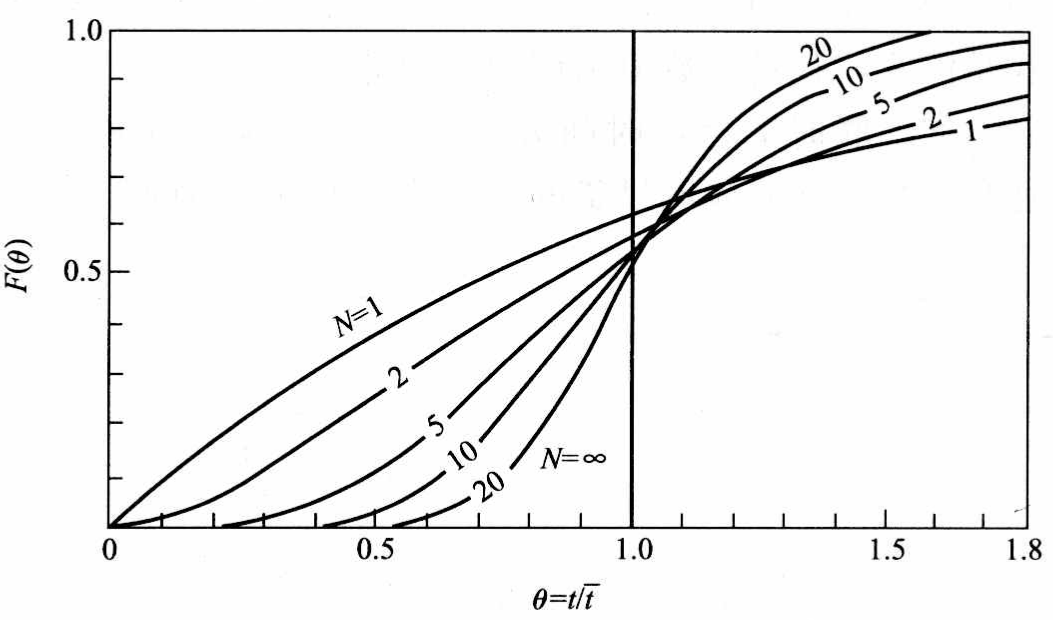
\includegraphics[width=.67\linewidth]{figures/fig5.18.png}
        \caption{多釜串联模型的$F(\theta)$图}
    \end{figure}    

\end{frame}


\begin{frame}
    \frametitle{多釜串联模型}

    将式$F(\theta)$对$\theta$求导，可得多釜串联模型的停留时间分布密度
    \[
        E(\theta)=\frac{N^{N}}{(N-1) !} \theta^{N-1} \mathrm{e}^{-N \theta}
    \]
    多釜串联模型的平均停留时间为
    \[
        \bar{\theta}=\int_{0}^{\infty} \frac{N^{N} \theta^{N} \mathrm{e}^{-N \theta}}{(N-1) !} \mathrm{d} \theta=1
    \]
    方差为
    \[
        \sigma_{\theta}^{2}=\int_{0}^{\infty} \frac{N^{N} \theta^{N+1} \mathrm{e}^{-N \theta}}{(N-1) !} \mathrm{d} \theta-1 =\frac{N+1}{N}-1=\frac{1}{N}
    \]
    当$N=1$时，$\sigma_{\theta}^{2}=1$，与全混流模型一致；而当$N=\infty$时，$\sigma_{\theta}^{2}=0$，与活塞流模型相一致。当N为任何正数时，其方差应介于0与1之间。

\end{frame}


\begin{frame}
    \frametitle{多釜串联模型}

    \begin{minipage}{0.52\linewidth}
        \begin{figure}        
            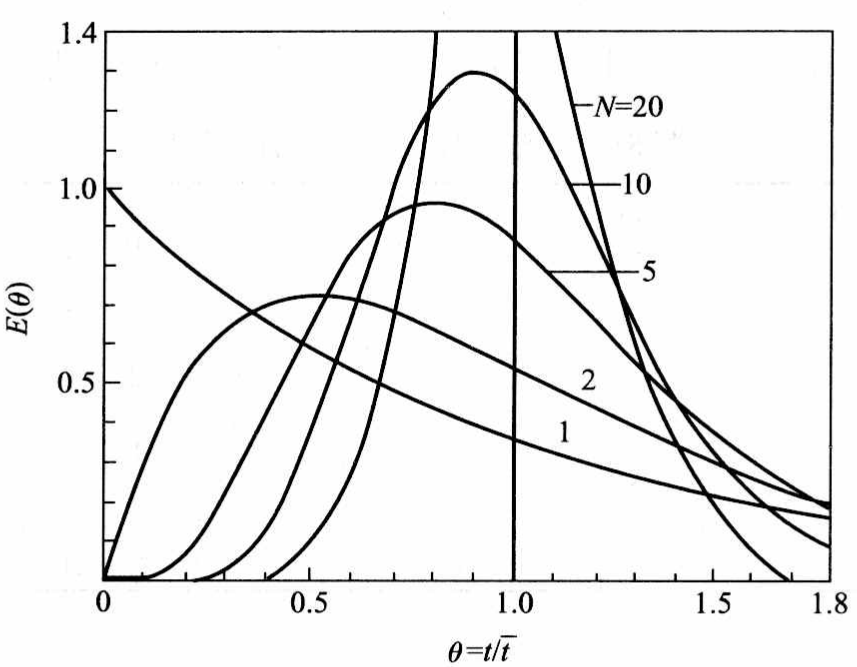
\includegraphics[width=\linewidth]{figures/fig5.19.png}
            \caption{多釜串联模型的$E(\theta)$图}
        \end{figure} 
    \end{minipage}\hfill
    \begin{minipage}{0.46\linewidth}
        \begin{itemize}
            \item $N$增加，停留时间分布变窄
        \end{itemize}
        \bigskip
        应用多釜串联模型来模拟一个实际反应器的流动状况时，首先要测定该反应器的停留时间分布，然后求出该分布的方差，将其代入$\sigma_{\theta}^{2}=\frac{1}{N}$便可算出模型参数N。
        \bigskip

        $N$为非整数？        
        \begin{itemize}
            \item 四舍五入
            \item 将小数部分视作小釜
        \end{itemize}
    \end{minipage}
     
\end{frame}


\begin{frame}[t]
    \frametitle{}
    \begin{example}
        以苯甲酸为示踪剂 ， 用脉冲法测定一反应体积为\SI{1735}{cm^3}的液相反应器的停留时间分布 。 液体流量为\SI{40.2}{cm^3/min}， 示踪剂用量4.95 g。不同时刻下出口液体中示踪物的浓度 $c(t)$ 如下表所示 。 若用多釜串联模型来模拟该反应器 ， 试求模型参数$N$。
        \begin{table}
            \centering
            \begin{tabular}{cc|cc|cc|cc}
                \bottomrule
                $t$/min & $c(t)\times 10^3$/(g/cm$^3$) & $t$ & $c(t)\times 10^3$ & $t$ & $c(t)\times 10^3$ & $t$ & $c(t)\times 10^3$   \\ \hline
                10 & 0     & 40 & 3.520 & 65 & 0.910 & 90 & 0.131  \\ 
                15 & 0.113 & 45 & 2.840 & 70 & 0.619 & 95 & 0.094  \\ 
                20 & 0.863 & 50 & 2.270 & 75 & 0.413 & 100 & 0.075  \\ 
                25 & 2.210 & 55 & 1.735 & 80 & 0.300 & 105 & 0.001  \\ 
                30 & 3.340 & 60 & 1.276 & 85 & 0.207 & 110 & 0  \\ 
                35 & 3.720 &  &  &  &  &  &  \\ \toprule
            \end{tabular}
        \end{table}
        \vspace{-5pt}
    \end{example}
\end{frame}


\begin{frame}
    \frametitle{轴向扩散模型}

    由于分子扩散、涡流扩散以及流速分布不均匀等原因，而使流动状况偏离理想流动时，可用轴向扩散模型来模拟，这对管式反应器尤为合适。该模型假定：
    \begin{enumerate}
        \item 流体以恒定的流速$u$通过系统；
        \item 垂直于流体运动方向的横截面上径向浓度分布均一，即径向混合达最大；
        \item 由于湍流混合、分子扩散以及流速分布等传递机理而产生的扩散，仅发生在流动方向（即轴向），并以轴向扩散系数$Da$表示这些因素的综合作用，且用费克定律加以描述。
    \end{enumerate}
    由于返混是逆着主流体流动方向进行，所以\highlight{扩散通量}(单位时间内通过垂直于扩散方向的单位截面积的扩散物质流量)
    \[
        J = - Da \frac{\partial c}{\partial Z}
    \]
    同时假定在同一反应器内轴向扩散系数不随时间及位置而变，其数值大小与反应器的结构、操作条件及流体性质有关。

\end{frame}


\begin{frame}
    \frametitle{轴向扩散模型}

    根据上述假设，可建立轴向扩散模型的数学模型方程。
    \begin{figure}
        \centering
        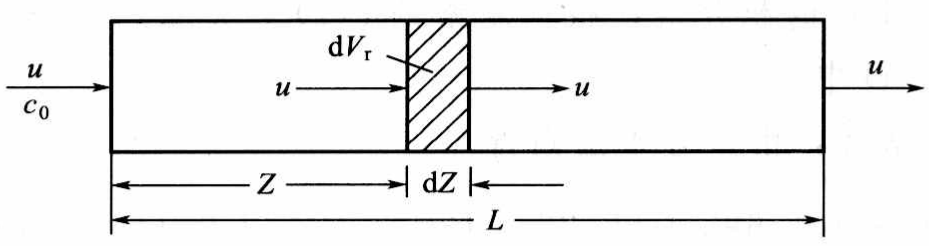
\includegraphics[width=\linewidth]{figures/fig5.20.png}
    \end{figure}
    取微元体积$\dif V_\mathrm{r}$作控制体积，对微元体积作示踪剂的物料衡算即得模型方程。

    若其横截面积为$A_\mathrm{r}$，则$\dif V_\mathrm{r} = A_\mathrm{r} \dif Z$。

\end{frame}


\begin{frame}
    \frametitle{轴向扩散模型}

    输入应包括两项，一是通过对流；另一是通过扩散。同样输出也应包括两项。
    \[
        \red{\text{输入}} = \magenta{\text{输出}} + \cyan{\text{累积}}
    \]
    \[
        \red{u A_{\mathrm{r}} c+D a A_{\mathrm{r}} \frac{\partial}{\partial Z}\left(c+\frac{\partial c}{\partial Z} \mathrm{~d} Z\right)} = \magenta{u A_{\mathrm{r}}\left(c+\frac{\partial c}{\partial Z} \mathrm{~d} Z\right)+D a A_{\mathrm{r}} \frac{\partial c}{\partial Z}
        } + \cyan{\frac{\partial c}{\partial t} A_{\mathrm{r}} \mathrm{d} Z}
    \]
    整理后，得
    \[
        \frac{\partial c}{\partial t}=D a \frac{\partial^{2} c}{\partial Z^{2}}-u \frac{\partial c}{\partial Z}
    \]
    此即轴向扩散模型方程。这里共有两个自变量，一是时间自变量$t$，另一为空间自变量，即轴向距离$Z$，所以模型方程为一偏微分方程。

    轴向扩散模型实质上是活塞流模型再迭加一扩散项，即上式右边第一项。通过此项反映系统内返混的大小。若$Da=0$，则化为活塞流模型方程
    \[
        \frac{\partial c}{\partial t}=-u \frac{\partial c}{\partial Z}
    \]
    \vspace{-10pt}
\end{frame}


\begin{frame}
    \frametitle{轴向扩散模型}

    通常将轴向扩散模型方程化为无量纲形式，这样使用起来比较方便。为此，引入下列各无因次量
    \[
        \theta=\frac{t u}{L_{\mathrm{r}}} \qquad \psi =\frac{c}{c_{0}} \qquad \zeta=\frac{Z}{L_{\mathrm{r}}} \qquad P e=\frac{u L_{\mathrm{r}}}{D a}
    \]
    轴向扩散模型无量纲方程为
    \[
        \frac{\partial \psi}{\partial \theta}=\frac{1}{P e} \frac{\partial^{2} \psi}{\partial \zeta^{2}}-\frac{\partial \psi}{\partial \zeta}
    \]
    $Pe$为贝克来数，其物理意义为
    \[
        P e=\frac{u L_{\mathrm{r}}}{D a}=\frac{\text { 对流传递速率 }}{\text { 扩散传递速率 }}
    \]
    贝克来数反映了返混的程度。$Pe$越大，返混程度越小。

\end{frame}


\begin{frame}
    \frametitle{轴向扩散模型}

    闭式系统，示踪剂以阶跃方式输入时，
    \[
        F(\theta)=1-\mathrm{e}^{P e / 2} \sum_{n=1}^{\infty} \frac{8 \omega_{\mathrm{n}} \sin \omega_{\mathrm{n}} \exp \left[-\left(P e^{2}+4 \omega_{\mathrm{n}}\right) \theta / 4 P e\right]}{P e^{2}+4 P e+4 \omega_{\mathrm{n}}^{2}}
    \]
    式中，$\omega_{\mathrm{n}}$为下列方程的正根
    \[
        \tan \omega_{\mathrm{n}}=\frac{4 \omega_{\mathrm{n}} P e}{4 \omega_{\mathrm{n}}^{2}-P e^{2}}
    \]
    \[
        E(\theta)=\mathrm{e}^{P e / 2} \sum_{n=1}^{\infty} \frac{(-1)^{\mathrm{n}+1} 8 \omega_{\mathrm{n}}^{2} \exp \left[-\left(P e^{2}+4 \omega_{\mathrm{n}}^{2}\right) \theta / 4 P e\right]}{P e^{2}+4 P e+4 \omega_{\mathrm{n}}^{2}}
    \]
    

\end{frame}


\begin{frame}
    \frametitle{轴向扩散模型}

    \begin{figure}
        \centering
        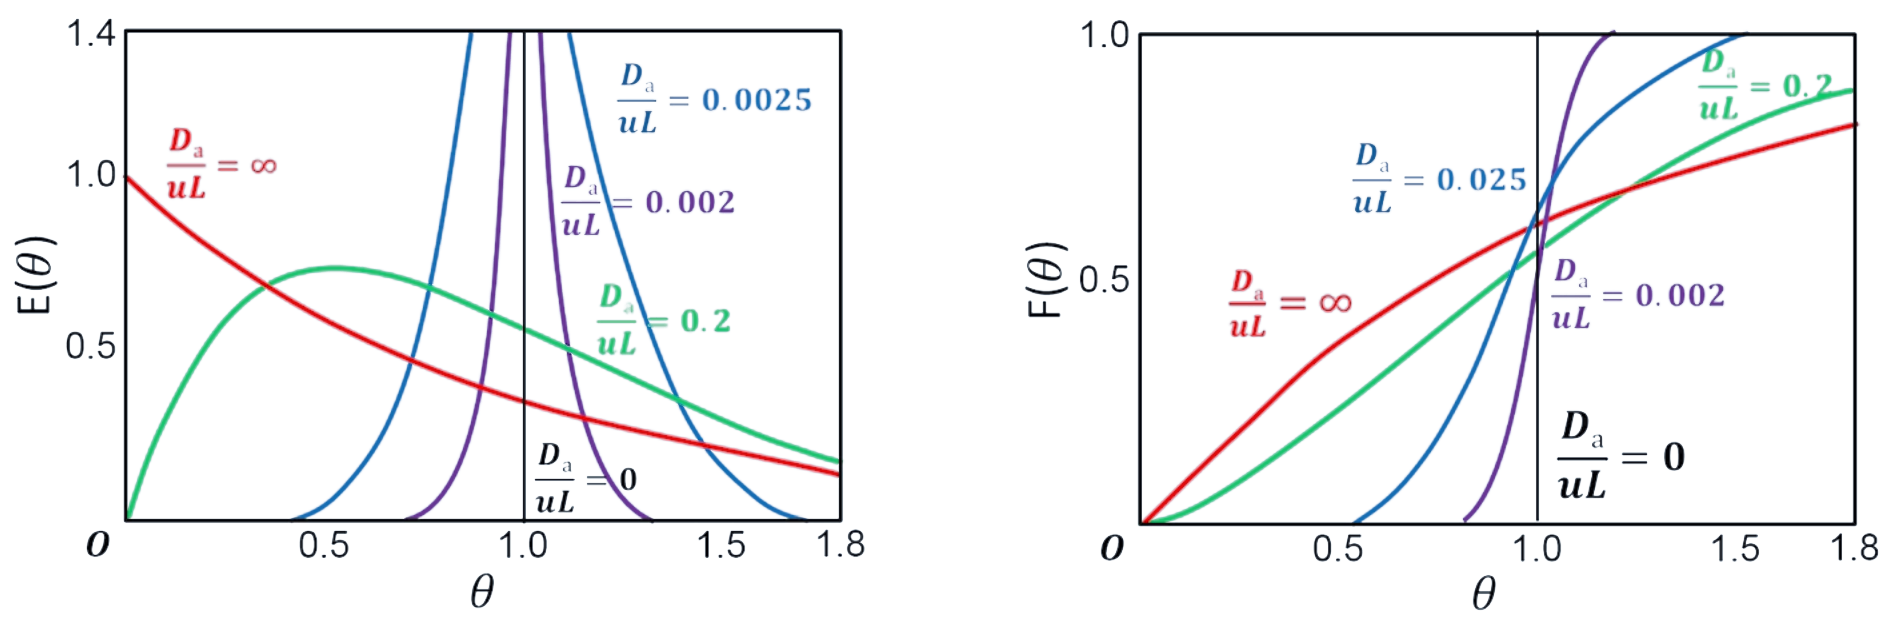
\includegraphics[width=\linewidth]{figures/fig5.21.png}
    \end{figure}
    随着模型参数$Pe$的倒数的减小，停留时间分布变窄。
    \begin{itemize}
        \item 当$Pe \to 0$时，属于全混流情况。
        \item 当$Pe \to \infty$时，属于活塞流情况
    \end{itemize}

\end{frame}


\begin{frame}
    \frametitle{轴向扩散模型}

    平均停留时间与方差为
    \[
        \bar \theta = 1
    \]
    \[
        \sigma_{\theta}^{2}=\frac{2}{P e}-\frac{2}{P e^{2}}(1-\mathrm{e}^{-P e})
    \]
    如果实际系统的停留时间分布已知，则可求出该分布的方差，代入上式试差即可求出模型参数。

    设计反应器时，停留时间分布未知，这可根据有关关联式来估算$Pe$。例如，对于空管反应器
    \[
        \frac{1}{Pe} = \frac{1}{Sc \cdot Re} + \frac{Re \cdot Sc}{192}
    \]
    若为湍流，则用
    \[
        Pe = Re^{0.125}
    \]

\end{frame}


\begin{frame}[t]
    \frametitle{}
    \begin{example}
        以苯甲酸为示踪剂 ， 用脉冲法测定一反应体积为\SI{1735}{cm^3}的液相反应器的停留时间分布 。 液体流量为\SI{40.2}{cm^3/min}， 示踪剂用量4.95 g。不同时刻下出口液体中示踪物的浓度 $c(t)$ 如下表所示 。 用轴向扩散模型来模拟该反应器 ， 试求模型参数$Pe$。
        \begin{table}
            \centering
            \begin{tabular}{cc|cc|cc|cc}
                \bottomrule
                $t$/min & $c(t)\times 10^3$/(g/cm$^3$) & $t$ & $c(t)\times 10^3$ & $t$ & $c(t)\times 10^3$ & $t$ & $c(t)\times 10^3$   \\ \hline
                10 & 0     & 40 & 3.520 & 65 & 0.910 & 90 & 0.131  \\ 
                15 & 0.113 & 45 & 2.840 & 70 & 0.619 & 95 & 0.094  \\ 
                20 & 0.863 & 50 & 2.270 & 75 & 0.413 & 100 & 0.075  \\ 
                25 & 2.210 & 55 & 1.735 & 80 & 0.300 & 105 & 0.001  \\ 
                30 & 3.340 & 60 & 1.276 & 85 & 0.207 & 110 & 0  \\ 
                35 & 3.720 &  &  &  &  &  &  \\ \toprule
            \end{tabular}
        \end{table}
        \vspace{-5pt}
    \end{example}
\end{frame}


